\lhead{\emph{Background}}
\chapter{Background}
This chapter presents first different research areas and topics related to this thesis. Then in the second part related works are presented and compaired.

\section{Research areas}
To get an overview of the topics of this project the research can be divided into three areas; Gesture based interaction, eyes-free interaction and sound localization. This project will mainly include the common topics of these areas but also specific topics in each area. A comparison of these are presented in a venn diagram \ref{fig:Venn}.

\begin{figure}[htbp]
	\centering
		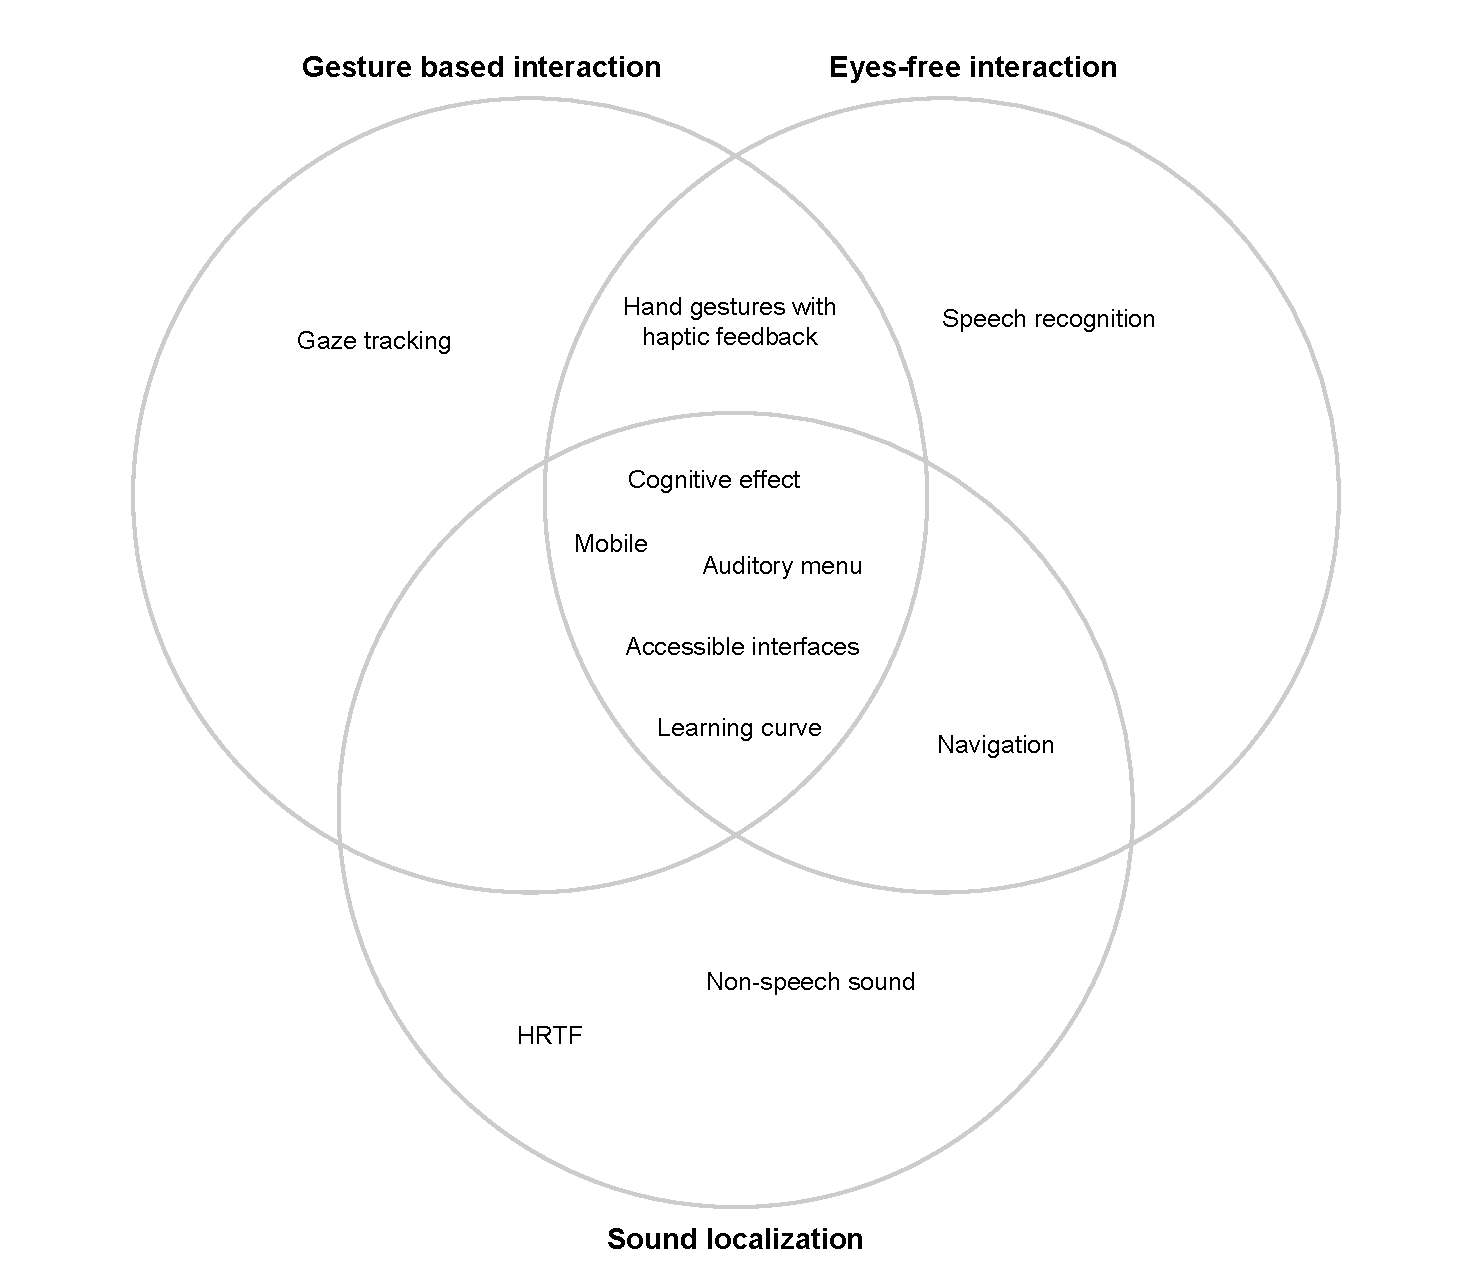
\includegraphics[width=\textwidth,height=\textheight,keepaspectratio]{./Figures/venn-diagram.pdf}
		\rule{35em}{0.5pt}
	\caption[Venn diagram]{A comparison of thesis topics}
	\label{fig:Venn}
\end{figure}

\subsection{Eyes-free interaction}
Several work on both audio \cite{kajastila_eyes-free_2013,bonner_no-look_2010,brewster_multimodaleyes-freeinteraction_2003,zhao_earpod:_2007,vazquez-alvarez_eyes-free_2011} and haptic \cite{pasquero_haptic_2011,pielot_tactile_2011} displays use the term eyes-free which refers to controlling the state of a system without visual attention. This kind of interaction has shown to be desirable in some situations \cite{oakley_designing_2007,yi_exploring_2012} and even improve efficiency compaired to traditional visual displays \cite{zhao_earpod:_2007}.

%Work on auditory [15, 12, 118] and haptic [86, 89] displays have used the term eyes-free, referring to the fact that the state of some system can be controlled or monitored without visual attention. Eyes-free interaction can take many forms, and in some situations it can be even faster than the visual counterparts [138]. The reasons why eyes-free interaction is needed or desirable [80, 138, 136] are discussed below:

\subsection{Gesture based interaction}
...

\subsection{Sound localization}
(Spatial audio, Head Related Transfer Function)...\\
Good reference for 3d sound \cite{begault_3dd_1994}

\section{Related work}
Based on the theories mentioned this section presents the research areas related to this thesis, the more specific related works in these areas and finally a sum up of the properties of the related works and this thesis.

% 1) intro - "in-the-field" interaction
Pascoe et al. investigated HCI issues when people are on the move and trials showed that a vital factor was to minimize the amount of distraction for interaction modes \cite{pascoe_using_2000}.

% 2) tendency on visual displays -> problems with this
Much of the interfaces work in wearable computing tends to focus on a visual headmounted displays \cite{barfield_fundamentals_2000} e.g. Google Project Glass. Visual displays can be obtrusive and hard to use in bright daylight, plus they occupy the users’ visual attention \cite{geelhoed_safety_2000}.

% 3) audio feedback instead of visual
By compairing visual and audio feedback when pushing buttons on the same GUI, Brewster showed that it was difficult for users to devote all their visual attention to an interface while walking, running og driving and that the interaction workload decreased with audio feedback \cite{brewster_overcoming_2002}.

% 4) spatial audio, auditory menus, non-speech audio
William W. Gaver, a pioneer in audio interfaces, has explored several aspects of using sound in interfaces including the intuitiveness of presenting complex information to users in the form of audio \cite{gaver_sonicfinder:_1989}. Similarly Graham explores the advantages in reaction time when using ”auditory icons” \cite{graham_use_1999}. In \cite{gaver_auditory_1986} Gaver presents the use of spatial sound icons. In doing so, he draws forward the unutilized potential of creating natural interaction through spatial audio.

Kajastila and Lokki has done a user study comparing auditory and visual menus controlled by the same free-hand gestures where the majority of the participants felt that an auditory circular menu was faster than a visual based menu \cite{kajastila_interaction_2013}.

Work has shown that non-speech audio is effective in improving the interaction with mobile devices \cite{pirhonen_gestural_2002, sawhney_nomadic_2000}

% 5) gesture based interaction, maybe some cluttering?
% maybe some gaze ref to start with...

% closely related to my project
Brewster et al. showed that novel interaction techniques based on sound and gesture can significantly improve the usability of a wearable device in particular under "eyes-free" mobile conditions and that head gestures was a successful interaction technique with egocentric sounds the most effective \cite{brewster_multimodaleyes-freeinteraction_2003}.

\subsection{Summing up: Project focus}
Table: Summing up references that handles specific research areas...














